\documentclass[11pt]{article}\usepackage[]{graphicx}\usepackage[]{color}
%% maxwidth is the original width if it is less than linewidth
%% otherwise use linewidth (to make sure the graphics do not exceed the margin)
\makeatletter
\def\maxwidth{ %
  \ifdim\Gin@nat@width>\linewidth
    \linewidth
  \else
    \Gin@nat@width
  \fi
}
\makeatother

\definecolor{fgcolor}{rgb}{0, 0, 0}
\newcommand{\hlnum}[1]{\textcolor[rgb]{0,0,0}{#1}}%
\newcommand{\hlstr}[1]{\textcolor[rgb]{0,0,1}{#1}}%
\newcommand{\hlcom}[1]{\textcolor[rgb]{0.443,0.478,0.702}{#1}}%
\newcommand{\hlopt}[1]{\textcolor[rgb]{0,0,0}{#1}}%
\newcommand{\hlstd}[1]{\textcolor[rgb]{0,0,0}{#1}}%
\newcommand{\hlkwa}[1]{\textcolor[rgb]{0.498,0,0.333}{\textbf{#1}}}%
\newcommand{\hlkwb}[1]{\textcolor[rgb]{0.498,0,0.333}{\textbf{#1}}}%
\newcommand{\hlkwc}[1]{\textcolor[rgb]{0.498,0,0.333}{\textbf{#1}}}%
\newcommand{\hlkwd}[1]{\textcolor[rgb]{0,0,0}{#1}}%
\let\hlipl\hlkwb

\usepackage{framed}
\makeatletter
\newenvironment{kframe}{%
 \def\at@end@of@kframe{}%
 \ifinner\ifhmode%
  \def\at@end@of@kframe{\end{minipage}}%
  \begin{minipage}{\columnwidth}%
 \fi\fi%
 \def\FrameCommand##1{\hskip\@totalleftmargin \hskip-\fboxsep
 \colorbox{shadecolor}{##1}\hskip-\fboxsep
     % There is no \\@totalrightmargin, so:
     \hskip-\linewidth \hskip-\@totalleftmargin \hskip\columnwidth}%
 \MakeFramed {\advance\hsize-\width
   \@totalleftmargin\z@ \linewidth\hsize
   \@setminipage}}%
 {\par\unskip\endMakeFramed%
 \at@end@of@kframe}
\makeatother

\definecolor{shadecolor}{rgb}{.97, .97, .97}
\definecolor{messagecolor}{rgb}{0, 0, 0}
\definecolor{warningcolor}{rgb}{1, 0, 1}
\definecolor{errorcolor}{rgb}{1, 0, 0}
\newenvironment{knitrout}{}{} % an empty environment to be redefined in TeX

\usepackage{alltt}
%\usepackage[paperheight = 11in, paperwidth = 8.5in, inner = 1.25in, outer = 1in, top = 1in, twosided]{geometry}
\usepackage[paperheight = 11in, paperwidth = 8.5in, left = 1in, right = 1in, top = 1in]{geometry}
% compact headers
\usepackage[compact]{titlesec}
\usepackage{titletoc}

% beautiful captions
\usepackage[small, bf]{caption}

% Math
\usepackage{amsmath}
\usepackage{amsfonts}
\def\V{{\rm V}\,}
\def\E{{\rm E}\,}

% Font
\usepackage[sc, osf]{mathpazo}
\linespread{1.05} % to accomodate palatino
\usepackage[T1]{fontenc} % accented chars, etc...

% Margin Notes
\usepackage{marginnote}

% framed boxes for code
\usepackage[framemethod=tikz]{mdframed}
\definecolor{lightgray}{gray}{0.65}


\newmdenv[innerlinewidth=0.5pt, roundcorner=4pt,linecolor=lightgray,innerleftmargin=6pt,
innerrightmargin=6pt,innertopmargin=6pt,innerbottommargin=6pt]{codedeclaration}

% Bibliography
\usepackage{natbib}
\renewcommand\bibname{References}

% MIDA Macros
\newcommand\M{\marginnote{\LARGE \sc M}\noindent}
\newcommand\I{\bigskip\marginnote{\LARGE \sc I \hspace{.02em}}\noindent}
\newcommand\D{\bigskip\marginnote{\LARGE \sc D}\noindent}
\newcommand\A{\bigskip\marginnote{\LARGE \sc A}\noindent}
\reversemarginpar

\title{Declaring and Diagnosing Research Designs \\ {\normalsize Book Proposal Sample Sections}}
\author{Graeme Blair \quad Jasper Cooper \quad Alexander Coppock \quad and Macartan Humphreys}
\IfFileExists{upquote.sty}{\usepackage{upquote}}{}
\begin{document}
\maketitle

\noindent This document includes three sample sections of \textit{Declaring and Diagnosing Reseach Designs}. The first two are entries in the Design Library (Part B) and the third is an entry in the Principles section (Part C).






\bigskip \bigskip

\tableofcontents

\clearpage
%\noindent {\sc design library} \\ 
\noindent {\it\Large Simple Random Sampling} \\

\addcontentsline{toc}{section}{Simple Random Sampling}

\noindent Often we are interested in features of a population, but data on the entire population is prohibitively expensive to collect. Instead, researchers obtain data on a small fraction of the population and use measurements taken on that sample to draw inferences about the population.

Imagine we seek to estimate the average political ideology of residents of the small town of Portola, California, on a left-right scale that varies from 1 (most liberal) to 7 (most conservative). We draw a simple random sample in which residents have an equal chance of inclusion in the study. It's a straightforward design, but formally declaring it will make it easy to assess its properties. \smallskip

\subsection*{Design Declaration}

\M Even for this most basic of designs, researchers bring to bear a background model of the world. As described in Chapter 1, the three elements of a model are the signature, probability distributions over variables, and functional equations among variables. The signature here is a specification of the variable of interest, $Y$, with a well defined domain (seven possible values between 1 and 7). In the code declaration below, we assume a uniform distribution over these 7 values. This choice is a speculation about the population distribution of $Y$; some features of the design diagnosis will depend on the choice of distribution. The functional equations seem absent here as there is only one variable in the model. We could consider an elaboration of the model that includes three variables: the true outcome, $Y$; the decision to measure the outcome, $M$; and the measured outcome, $Y^M$. We ignore this complication for now under the assumption that $Y = Y^M$, i.e., that $Y$ is measured perfectly. Finally, the model also includes information about the size of the population. Portola, California, has a population of approximately 2100 people as of 2010, so $N = 2100$.

\I Our inquiry is the population mean of $Y$: $\frac{1}{N} \sum_1^N Y_i = \bar{Y}$.

\D In simple random sampling, we draw a random sample without replacement of size $n$, where every member of the population has an equal probability of inclusion in the sample, $\frac{n}{N}$. When $N$ is very large relative to $n$, units are drawn approximately independently. In this design we measure $Y$ for $n=100$ units in the sample; the other $N-n$ units are not measured.

\A  We estimate the population mean with the sample mean estimator: $\widehat{\overline{Y}} = \frac{1}{n} \sum_1^n Y_i$. Even though our inquiry implies our answer should be a single number, an answer strategy typically also provides statistics that help us assess the uncertainty around that single number. To construct a 95\% confidence interval around our estimate, we calculate the standard error of the sample mean, then approximate the sampling distribution of the sample mean estimator using a formula that includes a finite population correction. In particular, we approximate the estimated sampling distribution by a $t$ distribution with $n - 1$ degrees of freedom. In the code for our answer strategy, we spell out each step in turn. 

\begin{codedeclaration}

\begin{knitrout}\small
\definecolor{shadecolor}{rgb}{1, 1, 1}\color{fgcolor}\begin{kframe}
\begin{alltt}
\hlcom{# Model -------------------------------------------------------------------------------}
\hlstd{N} \hlkwb{<-} \hlnum{2100}
\hlstd{population} \hlkwb{<-} \hlkwd{declare_population}\hlstd{(}\hlkwc{N} \hlstd{= N,} \hlkwc{Y} \hlstd{=} \hlkwd{sample}\hlstd{(}\hlnum{1}\hlopt{:}\hlnum{7}\hlstd{, N,} \hlkwc{replace} \hlstd{=} \hlnum{TRUE}\hlstd{))}
\hlstd{fixed_population} \hlkwb{<-} \hlkwd{population}\hlstd{()}

\hlcom{# Inquiry -----------------------------------------------------------------------------}
\hlstd{estimand} \hlkwb{<-} \hlkwd{declare_estimand}\hlstd{(}\hlkwc{Ybar} \hlstd{=} \hlkwd{mean}\hlstd{(Y))}

\hlcom{# Data Strategy -----------------------------------------------------------------------}
\hlstd{n} \hlkwb{<-} \hlnum{100}
\hlstd{sampling} \hlkwb{<-} \hlkwd{declare_sampling}\hlstd{(}\hlkwc{n} \hlstd{= n)}

\hlcom{# Answer Strategy ---------------------------------------------------------------------}
\hlstd{estimator} \hlkwb{<-} \hlkwd{declare_estimator}\hlstd{(}
  \hlkwc{estimator_function} \hlstd{=} \hlkwa{function}\hlstd{(}\hlkwc{data}\hlstd{) \{}
      \hlstd{est} \hlkwb{<-} \hlkwd{mean}\hlstd{(data}\hlopt{$}\hlstd{Y)}
      \hlstd{se}  \hlkwb{<-} \hlkwd{sd}\hlstd{(data}\hlopt{$}\hlstd{Y)} \hlopt{*} \hlkwd{sqrt}\hlstd{((N} \hlopt{/} \hlstd{n} \hlopt{-} \hlnum{1}\hlstd{)} \hlopt{/} \hlstd{(N} \hlopt{-} \hlnum{1}\hlstd{))}
      \hlstd{critical_value} \hlkwb{<-} \hlkwd{qt}\hlstd{(}\hlnum{0.975}\hlstd{,} \hlkwc{df} \hlstd{= n} \hlopt{-} \hlnum{1}\hlstd{)}
      \hlstd{ci_lower} \hlkwb{<-} \hlstd{est} \hlopt{-} \hlstd{critical_value} \hlopt{*} \hlstd{se}
      \hlstd{ci_upper} \hlkwb{<-} \hlstd{est} \hlopt{+} \hlstd{critical_value} \hlopt{*} \hlstd{se}
      \hlkwd{data.frame}\hlstd{(est, ci_lower, ci_upper)\},}
  \hlkwc{estimand} \hlstd{= estimand,}
  \hlkwc{label} \hlstd{=} \hlstr{"Sample Mean Estimator"}\hlstd{)}

\hlcom{# Design ------------------------------------------------------------------------------}
\hlstd{design} \hlkwb{<-} \hlkwd{declare_design}\hlstd{(fixed_population, estimand, sampling, estimator)}
\hlstd{diagnosands} \hlkwb{<-} \hlkwd{declare_diagnosands}\hlstd{(}
  \hlkwc{bias} \hlstd{=} \hlkwd{mean}\hlstd{(est} \hlopt{-} \hlstd{estimand),}
  \hlkwc{mean_est} \hlstd{=} \hlkwd{mean}\hlstd{(est),}
  \hlkwc{coverage} \hlstd{=} \hlkwd{mean}\hlstd{(ci_lower} \hlopt{<=} \hlstd{estimand} \hlopt{&} \hlstd{estimand} \hlopt{<=} \hlstd{ci_upper)}
  \hlstd{)}
\end{alltt}
\end{kframe}
\end{knitrout}

\end{codedeclaration}


\subsection*{Takeaways} 

With the design declared we can run a diagnosis and plot results from Monte Carlo simulations of the design:

\begin{codedeclaration}
\begin{knitrout}\small
\definecolor{shadecolor}{rgb}{1, 1, 1}\color{fgcolor}\begin{kframe}
\begin{alltt}
\hlstd{diagnosis} \hlkwb{<-} \hlkwd{diagnose_design}\hlstd{(}
  \hlstd{design,} \hlkwc{sims} \hlstd{=} \hlnum{10000}\hlstd{,} \hlkwc{bootstrap_sims} \hlstd{=} \hlnum{1000}\hlstd{,} \hlkwc{diagnosands} \hlstd{= diagnosands)}
\end{alltt}
\end{kframe}
\end{knitrout}
\end{codedeclaration}

% latex table generated in R 3.4.1 by xtable 1.8-2 package
% Fri Oct 20 22:47:46 2017
\begin{table}[ht]
\centering
\begin{tabular}{rrrrr}
  \hline
Mean Estimate & Bias & SE(Bias) & Coverage & SE(Coverage) \\ 
  \hline
3.92 & -0.00 & 0.00 & 0.95 & 0.00 \\ 
   \hline
\end{tabular}
\end{table}


\begin{knitrout}\small
\definecolor{shadecolor}{rgb}{1, 1, 1}\color{fgcolor}\begin{figure}
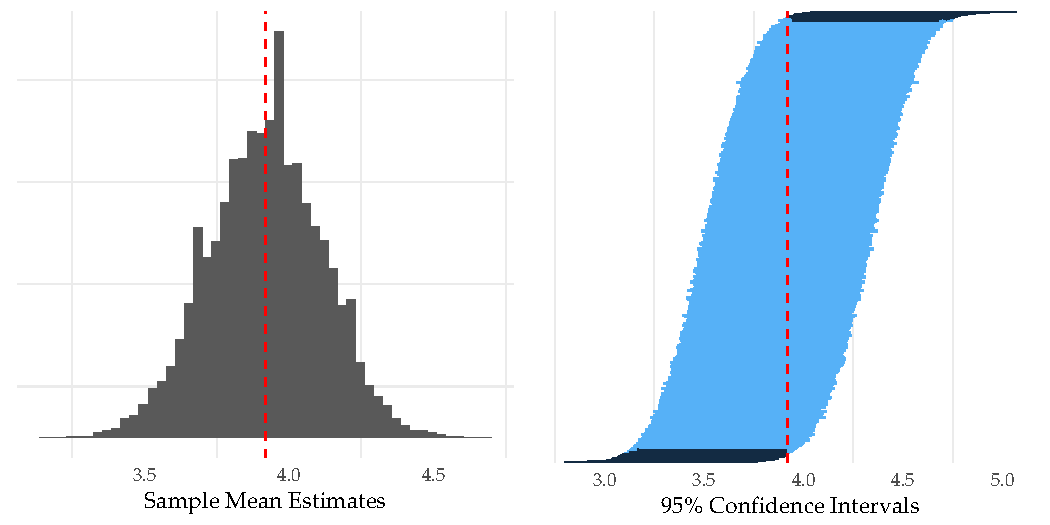
\includegraphics[width=\maxwidth]{figure/unnamed-chunk-6-1} \caption[Sampling Distributions of the Sample Mean and 95\% Confidence Interval]{Sampling Distributions of the Sample Mean and 95\% Confidence Interval}\label{fig:unnamed-chunk-6}
\end{figure}


\end{knitrout}

The diagnosis indicates that under simple random sampling, the sample mean estimator of the population mean is unbiased. The graph on the left shows the sampling distribution of the estimator: it's centered directly on the true value of the inquiry. Confidence intervals {\it also} have a sampling distribution -- they change depending on the idiosyncrasies of each sample we happen to draw. The figure on the right shows that the 95\% of the time the confidence intervals cover the true value of the estimand, as they should. As sample size grows, the sampling distribution of the estimator gets tighter, but the coverage of the confidence intervals stays at 95\% -- just the properties we would want out of our answer strategy.

Things work well here it seems. In the exercises we suggest some small modifications of the design that point to conditions under which things might break down.


\subsection*{Exercises} 

\begin{enumerate}
\item Modify the declaration to change the distribution of $Y$ from being uniform to something else: perhaps imagine that more extreme ideologies are more prevalent than moderate ones. Is the sample mean estimator still unbiased? Interpret your answer.
\item Change the sampling procedure to favor units with higher values of ideology. Is the sample mean estimator still unbiased? Interpret your answer.
\item Modify the estimation function to use this formula for the standard error: $\widehat{se} \equiv \frac{\widehat\sigma}{\sqrt{n}}$. This equation differs from the one used in our declaration (it ignores the total population size $N$). Check that the coverage of this new design is incorrect when $N=n$. Assess how large $N$ has to be for the difference between these procedures not to matter. 
\end{enumerate}

\clearpage
%\noindent {\sc design library} \\ 
\noindent {\it\Large Regression Discontinuity} \\
\addcontentsline{toc}{section}{Regression Discontinuity}


\noindent Regression discontinuity designs exploit substantive knowledge that treatment is assigned in a particular way: everyone above a threshold is assigned to treatment and everyone below it is not. Even though researchers do not control the assignment, substantive knowledge about the threshold serves as a basis for a strong identification claim.

Thistlewhite and Campbell introduced the regression discontinuity design in the 1960s to study the impact of scholarships on academic success. They claim that students with a test score just above a scholarship cutoff were plausibly comparable to students with scores just below the cutoff, so differences in future academic success could be attributed to the scholarship alone.

Regression discontinuity designs identify a {\it local} average treatment effect: the average effect of treatment {\it exactly at the cutoff}. The main trouble with the design is that there is vanishingly little data exactly at the cutoff, so any answer strategy needs to use data that is some distance away from the cutoff. The further away from the cutoff we move, the larger the threat of bias.

We consider a regression discontinuity design application that examines party incumbency advantage: the effect of a party winning an election on its vote margin in the next election. \smallskip

\subsection*{Design Declaration}

\M Regression discontinuity designs have four components: A running variable, a cutoff, a treatment variable, and an outcome. The cutoff determines which units are treated depending on the value of the running variable. In our example, the running variable $X$ is the Democratic party's margin of victory at time $t-1$; and the treatment, $Z$, is whether the Democratic party won the election in time $t-1$. The outcome, $Y$, is the Democratic vote margin at time $t$. We'll consider a population of 1,000 of these pairs of elections.
    
    \vspace{1em}
    
\hspace{2em}
\begin{knitrout}\small
\definecolor{shadecolor}{rgb}{1, 1, 1}\color{fgcolor}
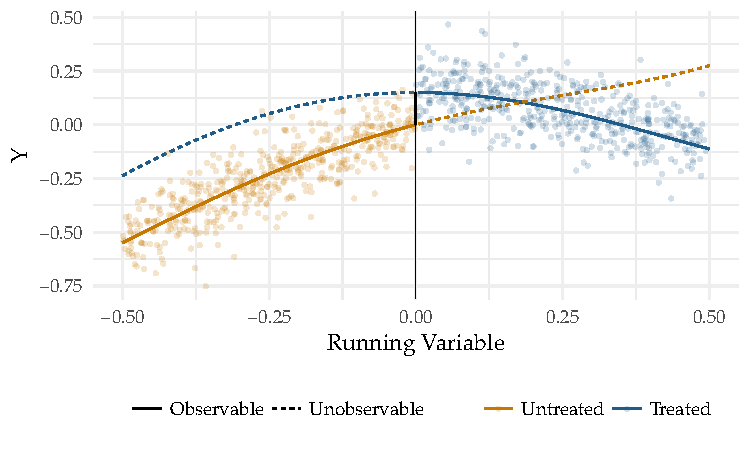
\includegraphics[width=\maxwidth]{figure/unnamed-chunk-7-1} 

\end{knitrout}


    
A major assumption required for regression discontinuity is that the conditional expectation functions for both treatment and control potential outcomes are continuous at the cutoff.\footnote{An alternative motivation for some designs that do not rely on continuity at the cutoff is "local randomization".} To satisfy this assumption, we specify two smooth conditional expectation functions, one for each potential outcome. The figure plots $Y$ (the Democratic vote margin at time $t$) against $X$ (the margin at time $t-1$). We've also plotted the true conditional expectation functions for the treated and control potential outcomes. The solid lines correspond to the observed data and the dashed lines correspond to the unobserved data.

\I Our estimand is the effect of a Democratic win in an election on the Democratic vote margin of the next election, when the Democratic vote margin of the first election is zero. Formally, it is the difference in the conditional expectation functions of control and treatment potential outcomes when the running variable is exactly zero. The plot's black vertical line shows this difference.

\D  We collect data on the Democratic vote share at time $t-1$ and time $t$ for all 1,000 pairs of elections. There is no sampling or random assignment.

\A We will approximate the treated and untreated conditional expectation functions to the left and right of the cutoff using a flexible regression specification estimated via OLS. In particular, we fit each regression using a fourth-order polynomial. Much of the literature on regression discontinuity designs focuses on the tradeoffs among answer strategies, with many analysts recommending against higher-order polynomial regression specifications. We use one here to highlight how well such an answer strategy does when it matches the functional form in the model. We discuss alternative estimators in the exercises. \begin{codedeclaration}
\begin{knitrout}\small
\definecolor{shadecolor}{rgb}{1, 1, 1}\color{fgcolor}\begin{kframe}
\begin{alltt}
\hlcom{# Model -------------------------------------------------------------------------------}
\hlstd{cutoff} \hlkwb{<-} \hlnum{.5}
\hlstd{control} \hlkwb{<-} \hlkwa{function}\hlstd{(}\hlkwc{X}\hlstd{) \{} \hlkwd{as.vector}\hlstd{(}\hlkwd{poly}\hlstd{(X,} \hlnum{4}\hlstd{,} \hlkwc{raw} \hlstd{= T)} \hlopt \hlkwd{c}\hlstd{(}\hlnum{.7}\hlstd{,} \hlopt{-}\hlnum{.8}\hlstd{,} \hlnum{.5}\hlstd{,} \hlnum{1}\hlstd{))\}}
\hlstd{treatment} \hlkwb{<-} \hlkwa{function}\hlstd{(}\hlkwc{X}\hlstd{) \{} \hlkwd{as.vector}\hlstd{(}\hlkwd{poly}\hlstd{(X,} \hlnum{4}\hlstd{,} \hlkwc{raw} \hlstd{= T)} \hlopt \hlkwd{c}\hlstd{(}\hlnum{0}\hlstd{,} \hlopt{-}\hlnum{1.5}\hlstd{,} \hlnum{.5}\hlstd{,} \hlnum{.8}\hlstd{))} \hlopt{+} \hlnum{.15}\hlstd{\}}
\hlstd{population} \hlkwb{<-} \hlkwd{declare_population}\hlstd{(}\hlkwc{N} \hlstd{=} \hlnum{1000}\hlstd{,}
  \hlkwc{X} \hlstd{=} \hlkwd{runif}\hlstd{(N,}\hlnum{0}\hlstd{,}\hlnum{1}\hlstd{)} \hlopt{-} \hlstd{cutoff,}
  \hlkwc{noise} \hlstd{=} \hlkwd{rnorm}\hlstd{(N,}\hlnum{0}\hlstd{,}\hlnum{.1}\hlstd{),}
  \hlkwc{Z} \hlstd{=} \hlnum{1} \hlopt{*} \hlstd{(X} \hlopt{>} \hlnum{0}\hlstd{))}
\hlstd{potential_outcomes} \hlkwb{<-} \hlkwd{declare_potential_outcomes}\hlstd{(}
  \hlkwc{Y_Z_0} \hlstd{=} \hlkwd{control}\hlstd{(X)} \hlopt{+} \hlstd{noise,}
  \hlkwc{Y_Z_1} \hlstd{=} \hlkwd{treatment}\hlstd{(X)} \hlopt{+} \hlstd{noise)}

\hlcom{# Inquiry -----------------------------------------------------------------------------}
\hlstd{estimand} \hlkwb{<-} \hlkwd{declare_estimand}\hlstd{(}\hlkwc{LATE} \hlstd{=} \hlkwd{treatment}\hlstd{(}\hlnum{0}\hlstd{)} \hlopt{-} \hlkwd{control}\hlstd{(}\hlnum{0}\hlstd{))}

\hlcom{# Answer Strategy ---------------------------------------------------------------------}
\hlstd{estimator} \hlkwb{<-} \hlkwd{declare_estimator}\hlstd{(Y} \hlopt{~} \hlkwd{poly}\hlstd{(X,} \hlnum{4}\hlstd{)} \hlopt{*} \hlstd{Z,}
                               \hlkwc{model} \hlstd{= lm,}
                               \hlkwc{estimand} \hlstd{= estimand)}

\hlcom{# Design ------------------------------------------------------------------------------}
\hlstd{design} \hlkwb{<-} \hlkwd{declare_design}\hlstd{(}
    \hlstd{population, potential_outcomes, estimand, reveal_outcomes, estimator)}
\end{alltt}
\end{kframe}
\end{knitrout}

\end{codedeclaration}


\subsection*{Takeaways} 

We now diagnose the design:
\begin{codedeclaration}
\begin{knitrout}\small
\definecolor{shadecolor}{rgb}{1, 1, 1}\color{fgcolor}\begin{kframe}
\begin{alltt}
\hlstd{diagnosis} \hlkwb{<-} \hlkwd{diagnose_design}\hlstd{(}
  \hlstd{design,} \hlkwc{sims} \hlstd{=} \hlnum{10000}\hlstd{,} \hlkwc{bootstrap_sims} \hlstd{=} \hlnum{1000}\hlstd{,} \hlkwc{diagnosands} \hlstd{= diagnosands)}
\end{alltt}
\end{kframe}
\end{knitrout}
\end{codedeclaration}

% latex table generated in R 3.4.1 by xtable 1.8-2 package
% Fri Oct 20 23:32:57 2017
\begin{table}[ht]
\centering
\begin{tabular}{rrrrrr}
  \hline
Bias & SE(Bias) & Power & SE(Power) & Coverage & SE(Coverage) \\ 
  \hline
-0.057 & 0.009 & 0.055 & 0.002 & 0.945 & 0.002 \\ 
   \hline
\end{tabular}
\end{table}



We highlight three takeaways. First, the power of this design is very low: with 1,000 units we do not achieve even 10\% statistical power. However, our estimates of the uncertainty are not too wide: the coverage probability indicates that our confidence intervals indeed contain the estimand 95\% of the time as they should. Our answer strategy is highly uncertain because the fourth-order polynomial specification in regression model gives weights to the data that greatly increase the variance of the estimator \citep{gelman2017high}. In the exercises we explore alternative answer strategies that perform better.
  
Second, the design is biased because polynomial approximations of the average effect at exactly the point of the threshold will be inaccurate in small samples~\citep{sekhontitiunik2017}, especially as units farther away from the cutoff are incorporated into the answer strategy. We know that the estimated bias is not due to simulation error by examining the bootstrapped standard error of the bias estimates.

Finally, from the figure, we can see how poorly the average effect at the threshold approximates the average effect for all units. The average treatment effect among the treated (to the right of the threshold in the figure) is negative, whereas at the threshold it is positive. This clarifies that the estimand of the regression discontinuity design, the difference at the cutoff, is only relevant for a small -- and possibly empty -- set of units very close to the cutoff. \smallskip

\subsection*{Further Reading} 

\begin{enumerate}
\item Since its rediscovery by social scientists in the late 1990s, the regression discontinuity design has been widely used to study diverse causal effects such as: prison on recidivism~\citep{Ojmarrh2017}; China's one child policy on human capital~\citep{qin2017}; eligibility for World Bank loans on political liberalization ~\citep{carnegie2017international}; and anti-discrimination laws on minority employment ~\citep{hahn1999evaluating}. 

\item We've discussed a ``sharp'' regression discontinuity design in which all units above the threshold were treated and all units below were untreated. In fuzzy regression discontinuity designs, some units above the cutoff remain untreated or some units below take treatment. This setting is analogous to experiments that experience noncompliance and may require instrumental variables approaches to the answer strategy (see {\bf Compliance is a Potential Outcome}).

\item Geographic regression discontinuity designs use distance to a border as the running variable: units on one side of the border are treated and units on the other are untreated. ~\citet{keele2016natural} use such a design to study whether voters are more likely to turn out when they have the opportunity to vote directly on legislation on so-called ballot initiatives. A complication of this design is how to measure distance to the border in two dimensions.
\end{enumerate}

\smallskip
\subsection*{Exercises}

\begin{enumerate}
\item \citet{gelman2017high} point out that higher order polynomial regression specifications lead to extreme regression weights. One approach to obtaining better estimates is to select a bandwidth, $h$, around the cutoff, and run a linear regression. Declare a sampling procedure that subsets the data to a bandwidth around the threshold, as well as a first order linear regression specification, and analyze how the power, bias, RMSE, and coverage of the design vary as a function of the bandwidth. 
  
\item The `rdrobust` estimator in the `rdrobust` package implements a local polynomial estimator that automatically selects a bandwidth for the RD analysis and bias-corrected confidence intervals. Declare another estimator using the `rdrobust` function and add it to the design. How does the coverage and bias of this estimator compare to the regression approaches declared above?

\item Reduce the number of polynomial terms of the the `treatment()` and `control()` functions and assess how the bias of the design changes as the potential outcomes become increasingly linear as a function of the running variable.
  
\item Redefine the population function so that units with higher potential outcome are more likely to locate just above the cutoff than below it. Assess whether and how this affects the bias of the design.
\end{enumerate}



\clearpage
%\noindent {\sc design principles} \\ 
\noindent {\it\Large Questions Should Have Answers} \\
\addcontentsline{toc}{section}{Questions Should Have Answers}

\noindent A basic requirement of a good research design is that the question it seeks to answer does in fact *have* an answer, at least under plausible models of the world. In our framework, this means that an inquiry $I$ must have an associated answer $a^M$, which refers to the answer under the model. Interestingly, we sometimes might not be conscious that the questions we ask do not have answers. Fortunately, when we ask a computer to answer such a question, it complains.

How could a question not have an answer? Answerless questions can arise when inquiries depend on variables that do not exist or are undefined for some units. In other words, when there is a mismatch between the model and the inquiry, we're asking a question about something that doesn't exist.

Consider an audit experiment (see {\bf Audit Experiment Design}) that seeks to assess the effects of an email from a Latino name (versus a White name) on {\it whether} and {\it how well} election officials respond to requests for information. For example, do they use a positive or negative tone. These questions seem reasonable enough. The problem, however, is that if there are officials who don't send responses, tone is undefined. More subtly, if there is an official that does send an email but would not have sent it in a different treatment condition, then tone is undefined for one of their potential outcomes.  \smallskip

\subsection*{Design Declaration}

\M The model has two outcome variables, $R_i$ and $Y_i$. $R_i$ stands for "response" and is equal to 1 if a response is sent, and 0 otherwise. $Y_i$ is the tone of the response and is normally distributed when it is defined. $Z_i$ is the treatment and equals 1 if the email is sent using a Latino name and 0 otherwise. The table below shows the potential outcomes for four possible types of subjects, depending on the potential outcomes of $R_i$. {\it A} types always respond regardless of treatment and {\it D} types never respond, regardless of treatment. {\it B} types respond if and only if they are treated, whereas {\it C} types respond if and only if they are {\it not} treated. The table also includes columns for the potential outcomes of $Y_i$, showing which potential outcome subjects would express depending on their type. The key thing to note is that for the B, C, and D types, the effect of treatment on $Y_i$ is {\it undefined} because messages never sent have no tone. The last (and very important) feature of our model is that the outcomes $Y_i$ are possibly correlated with subject type. Even though both $E[Y_i(1) | \text{Type} = A]$ and $E[Y_i(1) | \text{Type} = B]$ exist, there's no reason to expect that they are the same. 
    In the design we assume a distribution of types with  40\% {\it A}, 5\% {\it B}, 10\% {\it C}, and 45\% {\it D}.

\begin{table}[h]
\centering
\begin{tabular}{lllll}
   Type  &  $R_i(0)$  &  $R_i(1)$  &  $Y_i(0)$   &  $Y_i(1)$  \\ \hline
    A     &  1         &  1         &  $Y_i(0)$   &  $Y_i(1)$  \\
     B     &  0         &  1         &  NA         &  $Y_i(1)$  \\
     C     &  1         &  0         &  $Y_i(0)$   &  NA        \\
     D     &  0         &  0         &  NA         &  NA        
\end{tabular}
\caption{Causal Types}
\end{table}

\vspace{-1em}  \I We have two inquiries. The first is straightforward: $E[R_i(1) - R_i(0)]$ is the Average Treatment Effect on response. The second inquiry is the undefined inquiry that does not have an answer: $E[Y_i(1) - Y_i(0)]$. We will also consider a third inquiry, which {\it is} defined: $E[Y_i(1) - Y_i(0) | \mathrm{Type} = A]$, which is the average effect of treatment on tone among $A$ types.

\D The data strategy will be to use complete random assignment to assign 250 of 500 units to treatment.

\A We'll try to answer all three inquiries with the difference-in-means estimator, but as the diagnosis will reveal, this strategy works well for some inquiries but not others.

\begin{codedeclaration}

\begin{knitrout}\small
\definecolor{shadecolor}{rgb}{1, 1, 1}\color{fgcolor}\begin{kframe}
\begin{alltt}
\hlcom{# Model -------------------------------------------------------------------------------}
\hlstd{population} \hlkwb{<-} \hlkwd{declare_population}\hlstd{(}
  \hlkwc{N} \hlstd{=} \hlnum{500}\hlstd{,}
  \hlkwc{type} \hlstd{=} \hlkwd{sample}\hlstd{(}\hlkwd{c}\hlstd{(}\hlstr{"A"}\hlstd{,} \hlstr{"B"}\hlstd{,} \hlstr{"C"}\hlstd{,} \hlstr{"D"}\hlstd{),} \hlkwc{size} \hlstd{= N,}
                \hlkwc{replace} \hlstd{=} \hlnum{TRUE}\hlstd{,} \hlkwc{prob} \hlstd{=} \hlkwd{c}\hlstd{(}\hlnum{.40}\hlstd{,} \hlnum{.05}\hlstd{,} \hlnum{.10}\hlstd{,} \hlnum{.45}\hlstd{)))}

\hlstd{potential_outcomes} \hlkwb{<-} \hlkwd{declare_potential_outcomes}\hlstd{(}
  \hlkwc{R_Z_0} \hlstd{= type} \hlopt \hlkwd{c}\hlstd{(}\hlstr{"A"}\hlstd{,} \hlstr{"C"}\hlstd{),}
  \hlkwc{R_Z_1} \hlstd{= type} \hlopt \hlkwd{c}\hlstd{(}\hlstr{"A"}\hlstd{,} \hlstr{"B"}\hlstd{),}
  \hlkwc{Y_Z_0} \hlstd{=} \hlkwd{ifelse}\hlstd{(}
    \hlstd{R_Z_0,} \hlkwd{rnorm}\hlstd{(}\hlkwc{n} \hlstd{=} \hlkwd{sum}\hlstd{(R_Z_0),} \hlkwc{mean} \hlstd{=} \hlnum{.1}\hlopt{*}\hlstd{(type} \hlopt{==} \hlstr{"A"}\hlstd{)} \hlopt{-} \hlnum{2}\hlopt{*}\hlstd{(type} \hlopt{==} \hlstr{"C"}\hlstd{)),} \hlnum{NA}\hlstd{),}
  \hlkwc{Y_Z_1} \hlstd{=} \hlkwd{ifelse}\hlstd{(}
    \hlstd{R_Z_1,} \hlkwd{rnorm}\hlstd{(}\hlkwc{n} \hlstd{=} \hlkwd{sum}\hlstd{(R_Z_1),} \hlkwc{mean} \hlstd{=} \hlnum{.2}\hlopt{*}\hlstd{(type} \hlopt{==} \hlstr{"A"}\hlstd{)} \hlopt{+} \hlnum{2}\hlopt{*}\hlstd{(type} \hlopt{==} \hlstr{"B"}\hlstd{)),} \hlnum{NA}\hlstd{)}
\hlstd{)}

\hlcom{# Inquiry -----------------------------------------------------------------------------}
\hlstd{estimand_1} \hlkwb{<-} \hlkwd{declare_estimand}\hlstd{(}\hlkwc{ATE_R} \hlstd{=} \hlkwd{mean}\hlstd{(R_Z_1} \hlopt{-} \hlstd{R_Z_0))}
\hlstd{estimand_2} \hlkwb{<-} \hlkwd{declare_estimand}\hlstd{(}\hlkwc{ATE_Y} \hlstd{=} \hlkwd{mean}\hlstd{(Y_Z_1} \hlopt{-} \hlstd{Y_Z_0))}
\hlstd{estimand_3} \hlkwb{<-} \hlkwd{declare_estimand}\hlstd{(}
  \hlkwc{ATE_Y_for_As} \hlstd{=} \hlkwd{mean}\hlstd{(Y_Z_1[type} \hlopt{==} \hlstr{"A"}\hlstd{]} \hlopt{-} \hlstd{Y_Z_0[type} \hlopt{==} \hlstr{"A"}\hlstd{]))}

\hlcom{# Data Strategy -----------------------------------------------------------------------}
\hlstd{assignment} \hlkwb{<-} \hlkwd{declare_assignment}\hlstd{(}\hlkwc{m} \hlstd{=} \hlnum{250}\hlstd{)}

\hlcom{# Answer Strategy ---------------------------------------------------------------------}
\hlstd{estimator_1} \hlkwb{<-} \hlkwd{declare_estimator}\hlstd{(R} \hlopt{~} \hlstd{Z,} \hlkwc{estimand} \hlstd{= estimand_1,} \hlkwc{label} \hlstd{= ATE_R)}
\hlstd{estimator_2} \hlkwb{<-} \hlkwd{declare_estimator}\hlstd{(Y} \hlopt{~} \hlstd{Z,} \hlkwc{estimand} \hlstd{= estimand_2,} \hlkwc{label} \hlstd{= ATE_Y)}
\hlstd{estimator_3} \hlkwb{<-} \hlkwd{declare_estimator}\hlstd{(Y} \hlopt{~} \hlstd{Z,} \hlkwc{estimand} \hlstd{= estimand_3,} \hlkwc{label} \hlstd{= ATE_YA)}

\hlcom{# Design ------------------------------------------------------------------------------}
\hlstd{design} \hlkwb{<-} \hlkwd{declare_design}\hlstd{(}
  \hlstd{population,}
  \hlstd{potential_outcomes,}
  \hlstd{assignment,}
  \hlstd{estimand_1, estimand_2, estimand_3,}
  \hlkwd{reveal_outcomes}\hlstd{(}\hlkwc{outcome_variable_names} \hlstd{=} \hlkwd{c}\hlstd{(}\hlstr{"R"}\hlstd{,} \hlstr{"Y"}\hlstd{)),}
  \hlstd{estimator_1, estimator_2, estimator_3)}
\end{alltt}
\end{kframe}
\end{knitrout}

\end{codedeclaration}
\clearpage

\subsection*{Takeaways} 

We now diagnose the design:

\begin{codedeclaration}
\begin{knitrout}\small
\definecolor{shadecolor}{rgb}{1, 1, 1}\color{fgcolor}\begin{kframe}
\begin{alltt}
\hlstd{diagnosis} \hlkwb{<-} \hlkwd{diagnose_design}\hlstd{(}
  \hlstd{design,} \hlkwc{sims} \hlstd{=} \hlnum{10000}\hlstd{,} \hlkwc{bootstrap_sims} \hlstd{=} \hlnum{1000}\hlstd{,} \hlkwc{diagnosands} \hlstd{= diagnosands)}
\end{alltt}
\end{kframe}
\end{knitrout}
\end{codedeclaration}

% latex table generated in R 3.4.1 by xtable 1.8-2 package
% Fri Oct 20 23:19:51 2017
\begin{table}[ht]
\centering
\begin{tabular}{lrrrrr}
  \hline
Estimand Label & Mean Estimand & Mean Estimate & SE(Mean Estimate) & Bias & SE(Bias) \\ 
  \hline
ATE\_R & -0.05 & -0.05 & 0.00 & -0.00 & 0.00 \\ 
  ATE\_Y & NA & 0.52 & 0.00 & NA & NA \\ 
  ATE\_Y\_for\_As & 0.22 & 0.52 & 0.00 & 0.30 & 0.00 \\ 
   \hline
\end{tabular}
\end{table}


We learn three things from the design diagnosis. First, as expected, our experiment is unbiased for the average treatment effect on response.

Next, we see that our second inquiry, as well as our diagnostics for it, are undefined. The diagnosis tells us that our definition of potential outcomes produces a definition problem for the estimand. Note that the diagnosands that are defined, including power, depend only on the answer strategy and not on the estimand.

Finally, our third estimand -- the average effects for the $A$ types -- is defined but our estimates are biased. The reason for this is that we cannot tell from the data which types are the $A$ types: we are not conditioning on the correct subset. Indeed, we are unable to condition on the correct subset. If a subject responds in the treatment group, we don't know if she is an $A$ or a $B$ type; in the control group, we can't tell if a responder is an $A$ or a $C$ type. Our difference-in-means estimator of the ATE on $Y$ among $A$s will be off whenever $A$s have different outcomes from $B$s and $C$s.

In some cases, the problem might be resolved by changing the inquiry. Closely related estimands can often be defined, perhaps by redefining $Y$ (e.g., emails never sent have a tone of zero). Some redefinitions of the problem, as in the one we examine above, require estimating effects for unobserved subgroups which is a difficult challenge. 

\smallskip\subsection*{Applications}

This kind of problem is surprisingly common. Here are three more distinct instances of the problem:

\begin{enumerate}
\item $Y$ is the decision to vote Democrat ($Y=1$) or Republican ($Y=0$), $R$ is the decision to turn out to vote and $Z$ is a campaign message. The decision to vote may depend on treatment but if subjects do not vote then $Y$ is undefined.
\item $Y$ is the weight of infants, $R$ is whether a child is born and $Z$ is a maternal health intervention. Fertility may depend on treatment but the weight of unborn (possibly never conceived) babies is not defined.
\item $Y$ is the charity to whom contributions are made during fundraising and $R$ is whether anything is contributed and $Z$ is an encouragement to contribute. The identity of beneficiaries is not defined if there are no contributions. 
\end{enumerate}

All of these problem exhibit a form of post treatment bias (see section {\it Post treatment bias}) but the issue goes beyond picking the right estimator. Our problem here is conceptual: the effect of treatment on the outcome just doesn't exist for some subjects.


\smallskip \subsection*{Exercises} 

\begin{enumerate}
\item The amount of bias on the third estimand depends on both the distribution of types and the correlation of types with the potential outcomes of Y. Modify the declaration so that the estimator of the effect on Y is unbiased, changing only the distribution of types. Repeat the exercise, changing only the correlation of type with the potential outcomes of $Y$.  
\item Try approaching the problem by redefining the inquiry, seeking to assess the effect of treatment on the share of responses with positive tone. 
\end{enumerate}



\clearpage
\bibliographystyle{apsr}
\bibliography{ddrd.bib}

\end{document}
